%%
%% This is file `sample-acmlarge.tex',
%% generated with the docstrip utility.
%%
%% The original source files were:
%%
%% samples.dtx  (with options: `all,journal,bibtex,acmlarge')
%% 
%% IMPORTANT NOTICE:
%% 
%% For the copyright see the source file.
%% 
%% Any modified versions of this file must be renamed
%% with new filenames distinct from sample-acmlarge.tex.
%% 
%% For distribution of the original source see the terms
%% for copying and modification in the file samples.dtx.
%% 
%% This generated file may be distributed as long as the
%% original source files, as listed above, are part of the
%% same distribution. (The sources need not necessarily be
%% in the same archive or directory.)
%%
%%
%% Commands for TeXCount
%TC:macro \cite [option:text,text]
%TC:macro \citep [option:text,text]
%TC:macro \citet [option:text,text]
%TC:envir table 0 1
%TC:envir table* 0 1
%TC:envir tabular [ignore] word
%TC:envir displaymath 0 word
%TC:envir math 0 word
%TC:envir comment 0 0
%%
%% The first command in your LaTeX source must be the \documentclass
%% command.
%%
%% For submission and review of your manuscript please change the
%% command to \documentclass[manuscript, screen, review]{acmart}.
%%
%% When submitting camera ready or to TAPS, please change the command
%% to \documentclass[sigconf]{acmart} or whichever template is required
%% for your publication.
%%
%%
\documentclass[acmlarge]{acmart}
%%
%% \BibTeX command to typeset BibTeX logo in the docs
\AtBeginDocument{%
  \providecommand\BibTeX{{%
    Bib\TeX}}}

%% Rights management information.  This information is sent to you
%% when you complete the rights form.  These commands have SAMPLE
%% values in them; it is your responsibility as an author to replace
%% the commands and values with those provided to you when you
%% complete the rights form.
\setcopyright{acmlicensed}
\copyrightyear{2018}
\acmYear{2018}
\acmDOI{XXXXXXX.XXXXXXX}

%%
%% These commands are for a JOURNAL article.
\acmJournal{POMACS}
\acmVolume{37}
\acmNumber{4}
\acmArticle{111}
\acmMonth{8}

%%
%% Submission ID.
%% Use this when submitting an article to a sponsored event. You'll
%% receive a unique submission ID from the organizers
%% of the event, and this ID should be used as the parameter to this command.
%%\acmSubmissionID{123-A56-BU3}

%%
%% For managing citations, it is recommended to use bibliography
%% files in BibTeX format.
%%
%% You can then either use BibTeX with the ACM-Reference-Format style,
%% or BibLaTeX with the acmnumeric or acmauthoryear sytles, that include
%% support for advanced citation of software artefact from the
%% biblatex-software package, also separately available on CTAN.
%%
%% Look at the sample-*-biblatex.tex files for templates showcasing
%% the biblatex styles.
%%

\usepackage{subcaption}
\usepackage{caption}
\captionsetup[figure]{labelformat=empty}

%%
%% The majority of ACM publications use numbered citations and
%% references.  The command \citestyle{authoryear} switches to the
%% "author year" style.
%%
%% If you are preparing content for an event
%% sponsored by ACM SIGGRAPH, you must use the "author year" style of
%% citations and references.
%% Uncommenting
%% the next command will enable that style.
%%\citestyle{acmauthoryear}


%%
%% end of the preamble, start of the body of the document source.
\begin{document}

%%
%% The "title" command has an optional parameter,
%% allowing the author to define a "short title" to be used in page headers.
\title{Evaluating the Usability of Dynamically Moving Targets}

%%
%% The "author" command and its associated commands are used to define
%% the authors and their affiliations.
%% Of note is the shared affiliation of the first two authors, and the
%% "authornote" and "authornotemark" commands
%% used to denote shared contribution to the research.
\author{Rachel Xie}
\authornotemark[1]
\affiliation{%
  \institution{Colorado State University}
  \city{Fort Collins}
  \state{Colorado}
  \country{USA}
}

%%
%% By default, the full list of authors will be used in the page
%% headers. Often, this list is too long, and will overlap
%% other information printed in the page headers. This command allows
%% the author to define a more concise list
%% of authors' names for this purpose.
\renewcommand{\shortauthors}{Trovato et al.}

%%
%% The abstract is a short summary of the work to be presented in the
%% article.
\begin{abstract}
 This study investigates how dynamic targets affect user performance within the Fitts' Law framework by comparing four target conditions: static, growing, shrinking, and revolving targets. While Fitts' Law has been foundational in human-computer interaction for modeling pointing tasks with static targets, modern interfaces increasingly feature elements that change in size or position. Through a controlled experiment using a mouse-based target acquisition task, we measured movement time, accuracy, and error rates across the four conditions. Our findings reveal that traditional Fitts' Law models insufficiently capture the performance characteristics of dynamic targets, with growing targets maintaining performance similar to static targets while shrinking and moving targets significantly increased task difficulty beyond what Fitts' Law would predict. The results demonstrate the limitations of applying standard Fitts' Law to dynamic interactions and provide implications for interface design in gaming, medical applications, AR/VR environments, and other contexts where targets exhibit behaviors beyond the static paradigm upon which Fitts' Law was originally formulated.This research contributes to HCI theory by quantifying how spatial-temporal variability impacts pointing performance and offers a foundation for developing more accurate predictive models for contemporary interfaces.
\end{abstract}

%%
%% The code below is generated by the tool at http://dl.acm.org/ccs.cfm.
%% Please copy and paste the code instead of the example below.
%%
\begin{CCSXML}
<ccs2012>
 <concept>
  <concept_id>00000000.0000000.0000000</concept_id>
  <concept_significance>500</concept_significance>
 </concept>
 <concept>
  <concept_id>00000000.00000000.00000000</concept_id>
  <concept_desc>Do Not Use This Code, Generate the Correct Terms for Your Paper</concept_desc>
  <concept_significance>300</concept_significance>
 </concept>
 <concept>
  <concept_id>00000000.00000000.00000000</concept_id>
  <concept_desc>Do Not Use This Code, Generate the Correct Terms for Your Paper</concept_desc>
  <concept_significance>100</concept_significance>
 </concept>
 <concept>
  <concept_id>00000000.00000000.00000000</concept_id>
  <concept_desc>Do Not Use This Code, Generate the Correct Terms for Your Paper</concept_desc>
  <concept_significance>100</concept_significance>
 </concept>
</ccs2012>
\end{CCSXML}


\ccsdesc{Fitts' Law, Human-Computer Interaction, Dynamic Targets}


%%
%% Keywords. The author(s) should pick words that accurately describe
%% the work being presented. Separate the keywords with commas.
\keywords{Fitts' Law, Human-Computer Interaction, Dynamic Targets}



%%
%% This command processes the author and affiliation and title
%% information and builds the first part of the formatted document.
\maketitle

\section{Introduction}
Fitts’ Law, a cornerstone of human-computer interaction (HCI), has shaped the design of interfaces for decades by quantifying the relationship between movement time, target distance, and size. Formulated as the Index of Difficulty 
Fitts’ Law models the speed-accuracy tradeoff in human motor control. This model explains that larger or closer targets require less time, while smaller or farther targets demand greater precision and effort. Its applications span many domains, like optimizing graphical user interfaces (GUIs) and evaluating input devices like mice and touchscreens.

However, traditional Fitts’ Law studies predominantly focus on static targets that are fixed in size and position, despite modern interfaces where elements are dynamic, adaptive, or transient. Real world applications increasingly demand interactions with moving, growing, shrinking, or rotating targets: gamers fight enemies that dodge attacks, surgeons manipulate robotic arms to track shifting tissues in AR/VR environments, and drone controllers must track moving targets. These scenarios challenge the static assumptions of Fitts’ Law, leaving a gap in understanding how temporal-spatial variability impacts human accuracy.

This study bridges this gap by investigating how dynamic targets alter user accuracy and timing within the Fitts’ Law framework. We conduct a controlled experiment comparing performance across static, growing, shrinking, and revolving targets by varying target sizes and distances. By quantifying deviations from classical Fitts’ Law predictions, we explore whether existing models can be extended to account for dynamic conditions.

Through this experiment we will see how target motion impacts user accuracy and timing within the framework of Fitts’ Law. The findings aim to inform the design of dynamic interfaces, from gaming and AR/VR to adaptive robotics and training tools, while advancing HCI theory to better reflect real-world interactions of today’s technology

\section{Related Works}
The study of human-computer interaction (HCI) through the lens of Fitts’ Law has been extensive and has adapted to technological advancements and emerging interaction paradigms. Originally formulated to model pointing tasks in two-dimensional (2D) interfaces, Fitts’ Law remains an important law for evaluating speed-accuracy tradeoffs in motor control. Modern interfaces like virtual reality (VR), augmented reality (AR), gaming, and dynamic environments require more than this model. This section synthesizes research directions, focusing on adaptations of Fitts’ Law for novel interaction contexts, input device optimizations, and dynamic target behaviors. Prior work has advanced Fitts’ Law applications in VR, AR, training, and gaming. Many dynamic target studies focus on uni-dimensional behaviors (e.g., expansion or linear motion). This study explores this topic by evaluating diverse dynamic target types like static, growing, shrinking, revolving..

\subsection{Extensions to 3D and Growing Targets}
One area of research involves adapting Fitts’ Law to three-dimensional (3D) and immersive environments. Shi et al. (2023) pioneered this exploration in VR, investigating how target expansion affects selection performance using ISO 9241-411 tasks. Their study demonstrated that expanding target widths by 1.5× and 2.5× significantly reduced movement times, though error rates remained unaffected [1]. Similarly, Nwobodo et al. (2024) extended Fitts’ Law to AR by incorporating head movement dynamics and spatial orientation. By integrating quaternion algebra to model rotational distances and optimizing parameters via genetic algorithms, they reduced interaction task difficulty by 40 percent across quadrants, emphasizing the role of ergonomic object placement in AR interfaces [2]. These studies show necessity of redefining traditional metrics like "effective width", where angular displacement and depth perception alter interaction dynamics. 
\subsection{Input Device Sensitivity and Control-Display Gain}
The optimization of input devices, particularly in gaming and high-precision tasks, has revealed the relationships between control-display (CD) gain, movement time, and accuracy. Boudaoud et al. (2022) identified an optimal mouse sensitivity range (0.45–1.8°/mm) for first-person targeting tasks, linking performance degradation at high sensitivities to increased corrective submovements [3]. Their findings align with earlier work by Pang et al. (2019), who demonstrated that CD gain interacts with target amplitude and index of difficulty to account for ballistic versus visually controlled movements. The findings of  Pang et al. (2019) show that when using a computer mouse, different sensitivity settings work best depending on how far the target is. For small movements, a lower sensitivity (gain of 2.4) works best because it allows for more precise control. For larger movements across the screen, a higher sensitivity (gain of 14.5) is better [4]. These studies show the importance of balancing speed and precision in input device design, particularly in applications requiring rapid, repetitive actions, such as competitive gaming.
\subsection{Dynamic Targets}
Dynamic targets challenge the static assumptions of classical Fitts’ Law. Shi et al. (2023) examined target expansion in VR, showing that temporally increasing target width during cursor approach phases improved selection speed without compromising accuracy. This aligns with earlier 2D studies who found that growing targets reduced pointing times by effectively lowering the ID [1]. Dynamic behaviors introduce complexities such as predictive cursor adjustments and temporal uncertainty [5]. For instance, Yu et al. (2019) observed that revolving targets in VR required users to anticipate angular motion, suggesting that velocity and acceleration parameters could enhance Fitts’ Law models for moving targets. These findings show that there Fitts’ Law can be modified for dynamic targets.



\section{Methodology}
This study builds upon traditional Fitts’ Law by introducing dynamic targets to better understand user performance. This experiment varied target behavior across four conditions: static, growing, shrinking, and moving along a circular path. The target condition is the independent variable. Each condition was designed to simulate different levels of spatial complexity and motor control requirements, extending previous work on target acquisition in human-computer interaction.
Dynamic targets were inspired in part by applications in augmented and virtual reality, where target size and position often change in real time. Prior adaptations of Fitts’ Law in motion-rich environments show the importance of updating the law’s parameters to accommodate head movement, visual feedback, and spatial orientation[2].. By incorporating dynamic targets, this study aims to replicate similar motor-cognitive challenges in 2D interfaces, offering a bridge between classical HCI models and modern interaction systems.
\subsection{Participants}
A total of ten participants were selected for this research study, with ages ranging from 22 to 30. Seven identify as female and three identify as male. All of them are familiar with computer science principles, to varying degrees. These participants were recruited through my personal connections. The subjects received no incentives to participate in this study.
\subsection{Apparatus}
The experiment was implemented as a 3D Unity project deployed on a laptop computer. Participants used a standard computer mouse as the input device. The software was designed to present targets onto the screen according to the experimental conditions while recording timing and accuracy measurements. There is a central “start” button that is a blue circle which the subject will return to after selecting a target. The testing environment was controlled to minimize distractions, with consistent lighting and seating arrangements across all sessions.


\subsection{Experiment Design}
This study extends traditional Fitts' Law by introducing dynamic targets to investigate how target behavior affects user performance in pointing tasks. We employed a within-subjects design where each participant experienced all experimental conditions. Upon activation, a red target appears at one of the predetermined distances (200px or 322px) from the center point. The target is displayed at one of three fixed predetermined (20px, 40px, or 80px) and is randomly assigned one of four possible behaviors: static (control), growing (growing from 30\% to 100\% of original size over 2 seconds), shrinking (reducing from 100\% to 30\% of original size over 2 seconds), or moving in a small circular pattern (with a radius proportional to target size). If the user successfully hits the target, it changes color to green as visual feedback. In the case of a miss, a small red square marks the user's actual click location. In both cases, the start button will reappear and the subject will continue with the next target. For each trial, we measure three dependent variables: error rate (percentage of missed targets), movement time (milliseconds), and throughput (bits per second, calculated using the standard Index of Difficulty formula. A missed target will have 0 throughput but will be included in the average). These measurements are recorded and categorized according to the target's condition.

\section{Throughput Calculation}

In this experiment, throughput was calculated using the formula:

\begin{equation}
\text{Throughput} = \frac{\text{ID}}{\text{Movement Time (s)}} \text{ bits/s}
\end{equation}

where the Index of Difficulty (ID) was calculated using the Shannon formulation:

\begin{equation}
\text{ID} = \log_2\left(\frac{D}{W}+1\right) \text{ bits}
\end{equation}

with $D$ representing the distance to target and $W$ representing the target width. This differs from Fitts' original formulation:

\begin{equation}
\text{ID} = \log_2\left(\frac{2D}{W}\right) \text{ bits}
\end{equation}
\newline




\subsection{Procedure}
Subjects were shown a total of 45 targets with unlimited time to click each target. Each experimental session began with a brief explanation of the task and a demonstration of the different target behaviors. To begin the trial, the participant clicked the central blue start button. When the participant saw the target, they were instructed to click on the target and return to the central button afterwards, regardless of how accurate they were, and wait for the next target to appear. 
% \subsection{do i delete this}
% This experiment employed a within-subjects design to evaluate the impact of dynamic target behavior on pointing performance. The independent variable was target condition, with four levels:
% \begin{enumerate}
%     \item \textbf{Static} – the target remained stationary throughout the trial,
%     \item \textbf{Growing} – the target gradually increased from .3x to 1x of its size in 2 seconds,
%     \item \textbf{Shrinking} – the target gradually decreased 1x to .3x of its size in 2 seconds,
%     \item \textbf{Circular Motion} – the target continuously moved along a circular path.
% \end{enumerate}

% The primary dependent variables were:
% \begin{itemize}
%     \item \textbf{Movement Time (MT):} the time elapsed between clicking the start point and successfully selecting the target.
%     \item \textbf{Throughput:} the percentage of targets that the participant hit.
%     \item \textbf{Error Rate:} the proportion of targets in which the participant missed.
% \end{itemize}

These variables were chosen to assess both speed and precision, in line with Fitts’ Law principles. By comparing performance metrics across all target types within the same participants, the study aimed to determine how dynamic target behaviors influence pointing task difficulty.

\section{Results and Findings}


\begin{figure}[htbp]
    \centering
    \begin{tabular}{ccc}
        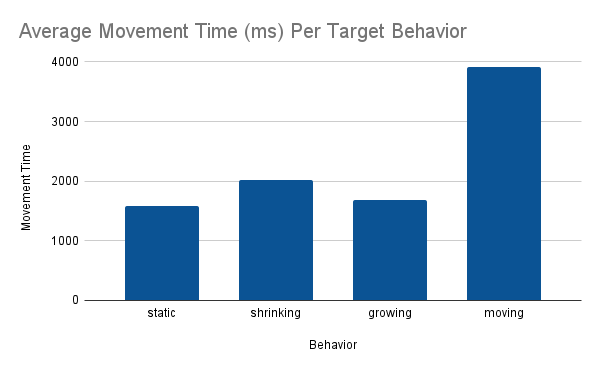
\includegraphics[width=0.3\textwidth, height=4cm]{Average Movement Time (ms) Per Target Behavior.png} &
        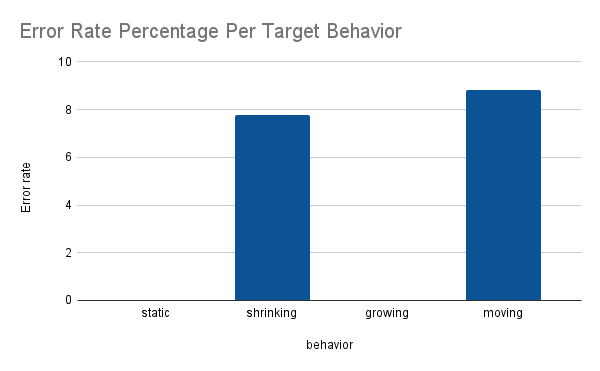
\includegraphics[width=0.3\textwidth, height=4cm]{Error Rate Percentage Per Target Behavior.png} &
        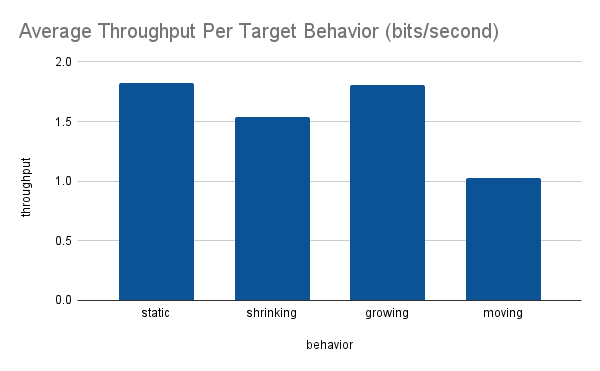
\includegraphics[width=0.3\textwidth, height=4cm]{Average Throughput Per Target Behavior (bits_second).png} \\
        (1) & (2) & (3) \\
    \end{tabular}
    \caption{}
\end{figure}

\begin{figure}[htbp]
    \centering
    \begin{tabular}{ccc}
        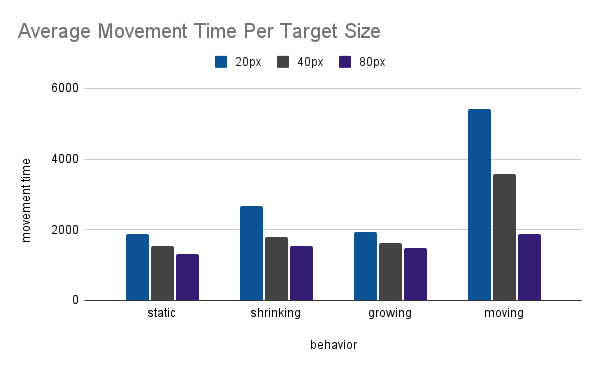
\includegraphics[width=0.3\textwidth, height=4cm]{Average Movement Time Per Target Size.png} &
        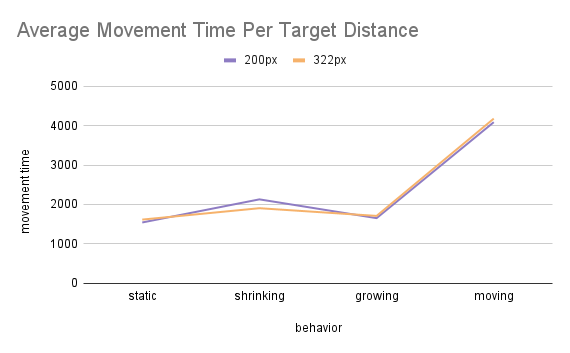
\includegraphics[width=0.3\textwidth, height=4cm]{Average Movement Time Per Target Distance.png} \\
        (4) & (5)  \\
    \end{tabular}
    \caption{}
\end{figure}





Data is analyzed from ten experimental trials with 45 participants each, comparing four different behaviors: static, shrinking, growing, and moving.We first examine overall effects of target behavior on movement time, error rates, and throughput, averaging across all sizes and distances to isolate the behavior effect (Figures 1-3). We then examine how target behavior interacts with target size (Figure 4) and distance (Figure 5). These analyses demonstrate that dynamic targets—particularly moving ones—not only increase task difficulty directly but also amplify the effects of other task parameters in ways that a standard Fitts' Law model fails to capture.


\subsection{Effect of Target Behavior on Performance}

The data collected shows that the target behavior significantly impacts pointing performance. Static targets established a baseline with an average movement time of 1582.89 ms (Figure 1). Growing targets performed comparably with only a 7\% increase in movement time, at 1689.48 ms. Shrinking targets showed a moderate degradation with a 28\% increase, at 2020.27 ms. Moving targets exhibited significantly worse performance, requiring 147\% more time, at 3919.25 ms compared to the static targets with the same pointing task.
	Error rates followed a similar pattern (Figure 2). Both static and growing targets maintained perfect accuracy with 0\% error rates across all experiments. Shrinking targets introduced moderate errors at 7.79\%, while moving targets resulted in the highest error rates of 8.83\%. This suggests that target behaviors requiring constant user adaptation increase the likelihood of failed selection attempts. 

\subsection{Throughput Evaluation}
Throughput measurements, which combine speed and accuracy into a single metric, revealed substantial differences between target behaviors (Figure 3). Static targets achieved the highest throughput (1.82 bits/s), followed closely by growing targets (1.81 bits/s). Shrinking targets showed a 15\% reduction in throughput (1.54 bits/s) compared to static targets, while moving targets exhibited a 43\% reduction (1.03 bits/s). This indicates that the information processing rate during target acquisition is significantly impaired by dynamic targets, particularly those in motion.

\subsection{Interaction between Target Size and Behavior}
Our results revealed that the effect of target size is amplified by dynamic behaviors (Figure 4). For static targets, small targets(20px) increased movement time by a moderate 42\% compared to large targets (80px). Growing targets showed even less sensitivity with only a 30\% increase. However, for shrinking targets, the increase was 73\%, and for moving targets, the increase was 188\%. This interaction effect is particularly notable, as it indicates that small targets become disproportionately more difficult when they also exhibit dynamic behavior. The combination of small size and movement created the most challenging condition, with small moving targets requiring over 5 seconds on average to select.
\subsection{Distance effects}
The impact of target distance varied considerably across behaviors. Static targets showed minimal distance sensitivity, with only a 5\% increase in movement time (Figure 5)for far targets (322px) compared to near targets (200px).Shrinking targets showed decrease in movement time (11\%), while moving targets were slightly affected by distance (2\% increase, though with considerably more variability).

Interestingly, for static and growing targets, throughput actually improved for farther distances, suggesting that users adopted more efficient movement strategies for longer distances. This pattern was reversed for shrinking and moving targets, where throughput declined with increased distance.

This variation in distance effects can be attributed to the fundamental difference between predictable and unpredictable target acquisition tasks. For static and growing targets, participants have movements guided by the well-established speed-accuracy trade-off described in traditional Fitts' Law. In these cases, participants can plan and execute a single, continuous movement to reach the target.

However, moving and shrinking targets introduce a constraint that fundamentally changes the nature of the task and thus increases the time needed to click on a target. The initial movement that serves participants well with static targets becomes less effective when the target's position is constantly changing. As the distance increases, participants must continuously update their aim to account for the target's changing position, which takes time. This creates a compounding effect where greater distances require both longer travel time and more complex trajectory adjustments.


\subsection{Practical Implications}

Our results have several important implications for interface design:

\begin{itemize}
   \item \textbf{Dynamic Feedback:} Growing elements (such as expanding buttons on hover) maintain good usability and may be implemented without significant performance costs. The minimal 7\% increase in movement time compared to static targets suggests that expanding interface elements can provide enhanced visual feedback without compromising efficiency.
   
   \item \textbf{Animations and Transitions:} Moving interface elements severely impact pointing performance, with movement times 147\% higher than static equivalents. Designers should minimize movement for elements requiring selection or provide mechanisms to pause animations during interaction. When movement is necessary, larger target sizes become essential to compensate for the increased difficulty.
   
   \item \textbf{Size Considerations:} Small targets (below 40px) should be avoided when implementing dynamic behaviors, as the combination creates disproportionate difficulty. Our data shows that while small static targets (20px) increased movement time by 42\% compared to large targets, this effect was amplified to 188\% for small moving targets. This interaction effect between size and behavior is particularly problematic for mobile interfaces where space constraints often lead to smaller targets.
   
   \item \textbf{Distance Sensitivity:} For moving targets, distance becomes a much more significant factor than for static targets. While static targets showed only a 5\% increase in movement time with greater distance, moving targets exhibited more pronounced effects and higher variability. Designers should place dynamic elements closer to likely cursor positions, especially when these elements are also small.
   
   \item \textbf{Error Tolerance:} Interfaces with necessarily dynamic elements should implement more generous error tolerance mechanisms, as error rates increase substantially with shrinking (7.79\%) and moving targets (8.83\%). This could include techniques such as expanding clickable areas beyond visible boundaries, implementing sticky targets, or providing temporary pausing of animations when the cursor approaches.
\end{itemize}

These implications are particularly relevant for interactive data visualizations, gaming interfaces, and dynamic content navigation systems where animated elements are common. Designers must carefully weigh the benefits of animation against the substantial costs to user performance when interaction with these elements is required.

\subsection{Limitations and Future Research}
While this study provides valuable insights, several limitations should be acknowledged. First, our experiment used a simplified target selection task that may not fully represent complex real-world interfaces. Second, we examined only four discrete behaviors, but real interfaces might exhibit combinations or variations of these behaviors.
Future research should explore additional dynamic behaviors (e.g., jittering, oscillating, accelerating), more complex trajectories for moving targets, and the effect of user-controlled versus system-controlled dynamics. Additionally, investigating how these effects change with different input devices (touchscreens, styluses, eye tracking) would further extend these findings.



\section{Conclusion}
This study investigated how dynamic targets affect user performance within the Fitts' Law framework, revealing differences across static, growing, shrinking, and revolving target conditions. Our findings demonstrate that traditional Fitts' Law models require some modification to account for target dynamism, with growing targets generally improving performance while shrinking and revolving targets increased task difficulty. Movement time and error rates were consistently affected by target behavior, suggesting that interface designers should consider these dynamics when optimizing user interactions.
The results have important implications for HCI theory and practice, particularly in contexts where targets change size or position such as gaming, medical applications, AR/VR environments, and drone control systems. By quantifying how dynamic targets affect pointing performance, this research extends traditional Fitts' Law understanding beyond static interactions and provides a foundation for more accurate predictive models in contemporary interfaces. Future work should explore additional dynamic behaviors, investigate combinations of multiple dynamic properties, and develop adaptive models that can account for varying levels of user expertise across different dynamic contexts. As interfaces continue to evolve toward more natural and fluid interactions, understanding the relationship between target dynamics and user performance becomes increasingly crucial for creating intuitive and effective human-computer interfaces.




\newpage
\begin{thebibliography}{99}

\bibitem{shi2023}
R.~Shi, Y.~Wei, Y.~Li, L.~Yu, and H.-N.~Liang, ``Expanding Targets in Virtual Reality Environments: A Fitts’ Law Study,'' in \textit{Proc. IEEE Int. Symp. on Mixed and Augmented Reality Adjunct (ISMAR-Adjunct)}, Sydney, Australia, 2023, pp. 615--618, doi: \href{https://doi.org/10.1109/ISMAR-Adjunct60411.2023.00132}{10.1109/ISMAR-Adjunct60411.2023.00132}.

\bibitem{nwobodo2024}
O.~J.~Nwobodo, K.~Wereszczyński, G.~S.~Kuaban, P.~Skurowski, and K.~A.~Cyran, ``An Adaptation of Fitts’ Law for Performance Evaluation and Optimization of Augmented Reality (AR) Interfaces,'' \textit{IEEE Access}, vol.~12, pp.~169614--169627, 2024, doi: \href{https://doi.org/10.1109/ACCESS.2024.3498444}{10.1109/ACCESS.2024.3498444}.

\bibitem{boudaoud2022}
B.~Boudaoud, J.~Spjut, and J.~Kim, ``Mouse Sensitivity in First-person Targeting Tasks,'' in \textit{Proc. IEEE Conf. on Games (CoG)}, Beijing, China, 2022, pp.~183--190, doi: \href{https://doi.org/10.1109/CoG51982.2022.9893626}{10.1109/CoG51982.2022.9893626}.

\bibitem{pang2019}
Y.~H.~Pang, E.~R.~Hoffmann, and R.~S.~Goonetilleke, ``Effects of Gain and Index of Difficulty on Mouse Movement Time and Fitts’ Law,'' \textit{IEEE Transactions on Human-Machine Systems}, vol.~49, no.~6, pp.~684--691, Dec.~2019, doi: \href{https://doi.org/10.1109/THMS.2019.2931743}{10.1109/THMS.2019.2931743}.

\bibitem{yu2018}
D.~Yu, H.-N.~Liang, F.~Lu, V.~Nanjappan, K.~Papangelis, and W.~Wang, ``Target selection in head-mounted display virtual reality environments,'' \textit{Journal of Universal Computer Science}, vol.~24, no.~9, pp.~1217--1243, 2018, doi: \href{https://doi.org/10.3217/jucs-024-09-1217}{10.3217/jucs-024-09-1217}.

\end{thebibliography}

\end{thebibliography}
\end{document}

\end{document}
\endinput
%%
%% End of file `sample-acmlarge.tex'.
